\documentclass{proc}

\usepackage{edbkps}
\usepackage{amsmath}
\usepackage{amssymb}
\usepackage{setspace}
\usepackage[utf8]{inputenc}
\usepackage{setspace}
\usepackage{subfig}
%%\usepackage[lined,boxed,commentsnumbered, linesnumbered]{algorithm2e}



\setcounter{secnumdepth}{2}
\setcounter{tocdepth}{0}
\let\footnote\savefootnote
\let\footnotetext\savefootnotetext
\let\footnoterule\savefootnoterule
\normallatexbib
\makeatletter
\renewcommand{\@ptsize}{0}
\makeatother

%%%%%
%% If you use a font encoding package, please enter it here, i.e.,
\usepackage{t1enc}


%%%%%
% Style for inserting .eps files and rotating illustrations or tables

% possible options for graphicx:
% [dvips], [xdvi], [dvipdf], [dvipsone], [dviwindo], [emtex], [dviwin],
% [pctexps],  [pctexwin],  [pctexhp],  [pctex32], [truetex], [tcidvi],
% [oztex], [textures]

\usepackage[dvips]{graphicx}
\usepackage[x11names, rgb]{xcolor}
\usepackage{tikz}
\usetikzlibrary{snakes,arrows,shapes}
\usepackage{amsmath}

%%%%%%%%%%%%%%%%%%%%%%%%%%%%%%%%%%%%%%%%%%%%%%%%%%%%%%%%%%%%%%%%%%%%%%%%%

\begin{document}


\articletitle[The Set Covering problem]
{Otimização no rank-1 de Chvátal-Gomory para o problema Set Covering}

\author{João C. Abreu\altaffilmark{1}}

\altaffiltext{1}{Universidade Federal de Minas Gerais, DCC, \\
Avenida Antônio Carlos 6627, Belo Horizonte, Brazil,\\
\email{joao.junior@dcc.ufmg.br}}

\anxx{João C. Abreu Jr.,Universidade Federal de Minas Gerais\,
Avenida Antônio Carlos 6627\, Belo Horizonte\, Brasil\,
\emailfont{joao.junior@dcc.ufmg.br}}

\begin{abstract}
Esse trabalho apresenta o problema Set Covering e um algoritmo para gerar todos os cortes de rank-1 de Chvátal-Gomory para esse problema.

\end{abstract}

\begin{keywords}
\inx{Set Covering}, \inx{Chvátal-Gomory}, \inx{Desigualdades válidas}
\end{keywords}

\doublespacing

\section{Introdução}
\label{sec:intro}

Dados $M=\{1,...,m\}$ e $N=\{1,...,n\}$ dois conjuntos. Seja $M_1$, $M_2$, ..., $M_n$ uma coleção de subconjuntos 
de $M$ com um custo $c_j$ associado a cada um desses subconjuntos. Uma cobertura de $M$ é um subconjunto 
$F \subset N$ tal que $\cup_{j \in F} M_j = M$. O problema que consiste em encontrar esse subconjunto $F \subset N$ de custo mínimo
é denominado o problema Set Covering($SCP$). Segundo Balas\cite{balas89} esse problema é $np$-$dificil$ e não se conhece uma boa caracterização do politopo desse
problema. \\
Em \cite{balas89}, Balas caracteriza a classe de inequações válidas para o $SCP$ com coeficientes iguais a 0,1 ou 2 e apresenta condições 
necessárias e suficientes para essas restrições serem não dominadas por outras. Esse paper também mostra que todas as inequações desse tipo são
às únicas a formarem o feixo 1 de Chvátal-Gomory. \\
Em \cite{saxena04} Saxena extende o trabalho de Balas\cite{balas89} e apresenta uma caracterização da classe de inequações válidas para o $SCP$ com 
coeficientes iguais a 0, 1, 2 ou 3 e propõe um problema $np$-$dificil$ para gerar todas essas inequações a partir de soluções fracionárias
do $SCP$. \\
Em \cite{Beasley87}, Beasley propõe um algoritmo para resolver o $SCP$ baseado nos resultados teóricos propostos em \cite{balas89}. \\
O Objetivo desse trabalho é otimizar o problema $SCP$ através do rank-1 de Chvátal-Gomory. A seção \ref{sec:modelagem} apresenta uma modelagem
matemática para esse problema, a seção \ref{sec:algoritmo} apresenta um algoritmo para gerar as restrições Chvátal-Gomory de rank1 e resolver
o $SCP$ com essas restrições, a seção \ref{sec:exemplo} apresenta um pequeno exemplo da utilização do algoritmo proposto na seção 
\ref{sec:algoritmo},
a seção \ref{sec:experimentos} apresenta os experimentos computacionais obtidos aplicando o algoritmo da seção \ref{sec:algoritmo} nas instâncias presentes na literatura e
a seção \ref{sec:consideracoes} apresenta as conclusões. 

\section{Modelagem Matematica}\label{sec:modelagem} 
Essa seção apresenta a formulação para o $SCP$ proposta em \cite{Bertsimas05}. Para formular o SCP como um problema
de otimização inteira, é introduzida uma matriz de incidência $A$ de tamanho $mxn$ para a coleção de subconjuntos 
$M_j, \forall j \in N$, com as entradas dadas por: \
\begin{align}
    & a_{ij} = \left \{\begin{array}{ll} 1; & \textrm{se } i \in M_j \textrm{,} \nonumber \\
    0; & \textrm{caso contrário} \nonumber \label{eq:fluxo}
    \end{array}\right. \\
\end{align}
Nessa formulação, a função objetivo \eqref{eq:objetivo} minimiza o custo da cobertura procurada. 
Os valores constantes $c_j, \forall j \in N$ são os custos de cada subconjunto $M_j$. 
A variável de decisão $x_j$ é igual a $1$ quando $j \in F$ e $0$, caso contrário, onde $F \subset N$ é a cobertura procurada. \\
\begin{align}
    & \text{min } \sum_{j \in N} c_jx_j \label{eq:objetivo} \\
    & \text{Sujeito à:} \nonumber \\
    & Ax \ge 1 \\
    & x \in \{0,1\}^n \label{eq:binarias}
\end{align}

\section{Algoritmo}\label{sec:algoritmo} 
Essa seção apresenta um algoritmo para gerar todos os cortes de Chvátal-Gomory de rank-1 e foi retirado
de \cite{Fischetti07}. A figura \ref{AlgoritmoRank1} apresenta esse algoritmo. Na linha 2 o modelo da seção
\ref{sec:modelagem} é relaxado, isto é, as variáveis $x$ agora pertencem ao intervalo $[0,1]$, e então é 
resolvido. Os laços das linhas 3 a 10 são executados até que uma solução inteira seja encontrada ou 
que o tempo máximo ocorra. A linha 3 verifica se a atual solução $x$ é inteira, caso positivo, nada mais 
precisa ser feito, caso negativo entra-se no loop. A linha 4 verifica se existe algum corte de 
Chvátal-Gomory de rank-1 que corta $x$, caso positivo a linha 5 adiciona o corte encontrado no 
modelo relaxado e a linha 6 resolve o modelo relaxado com esse novo corte. Caso nenhum corte seja
encontrado a linha 9 é executada e o algoritmo termina.
\begin{figure}
\centering
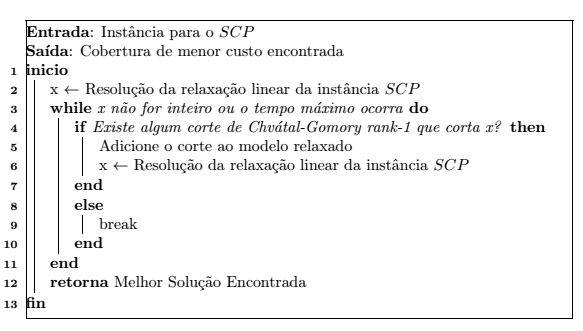
\includegraphics[width=4in]{AlgoritmoRank1.PNG}
\caption{Algoritmo para encontrar cortes de Chvátal-Gomory de rank-1 para o $SCP$}
\label{AlgoritmoRank1}
\end{figure}
Para verificar se existe algum corte de Chvátal-Gomory de rank-1 que corta uma solução fracionária
$x$ é utilizado um formulação de programação linear inteira mista baseada na formulação do problema de separação $np$-$dificil$ proposta em
\cite{Fischetti07}. A formulação
é composta pela função objetivo \eqref{eq:objetivo} e pelas restrições \eqref{eq:resticaoA}-\eqref{eq:inteira}.
\begin{align}
    & \text{min } \sum_{j \in N} \alpha_jx_j - \alpha_0 \label{eq:objetivo} \\
    & \text{Sujeito à:} \nonumber \\
    & 0 \le \alpha_j - u^TA_j  \le 1 -\delta \textrm{,} \forall j \in N \label{eq:resticaoA} \\ 
    & 0 \le \alpha_0 - u^Tb \le 1 -\delta \label{eq:b} \\
    & 0 \le u_i \le 1 -\delta \textrm{,} \forall i=1,...,m \label{eq:u} \\
    & \alpha_0 \le \sum_{j \in N} \alpha_j \textrm{,} \label{eq:mantem_binarias} \\
    & \alpha_0, \alpha_j \textrm{ inteiro, } \forall j \in N \label{eq:inteira}
\end{align}
Dada uma solução fracionária $x$ para o $SCP$, se a formulação anterior possui solução negativa,
então teremos $ \lceil u^TA_j \rceil x_j \le \lceil u^Tb \rceil$, então a restrição
$ \lceil u^TA_j \rceil x_j \ge \lceil u^Tb \rceil$ é um restrição válida para o $SCP$ que corta $x$. A restrição \eqref{eq:resticaoA},
juntamente com a restrição \eqref{eq:inteira} garantem que $\alpha_j$ é o menor inteiro, maior ou igual a $u^TA_j$,
ou seja $\alpha_j = \lceil u^TA_j \rceil$.
A restrição \eqref{eq:b},
juntamente com a restrição \eqref{eq:inteira} garantem que $\alpha_0$ é o menor inteiro, maior ou igual a $u^Tb$, ou seja
$\alpha_0 = \lceil u^Tb \rceil$. A restrição \eqref{eq:mantem_binarias} garante que os cortes gerados continuaram
a manter as variáveis $x$ com um valor máximo 1.

\section{Exemplo}\label{sec:exemplo} 
Essa seção apresenta uma pequena instância para o problema $SCP$. Essa instância é então 
passada como entrada para o algoritmo da seção \ref{sec:algoritmo} e também é estudada com o software PORTA.
Para essa instância, o conjunto $M=\{1,2,3,4\}$ e o conjunto $N=\{1,2,3,4,5,6\}$. A matriz de incidência
$A$ para a coleção dos subconjuntos $M_j, \forall j \in N$ é dada abaixo.
$$
\begin{pmatrix} 
    1 & 0 & 1 & 0 & 0 & 1 \\ 
    0 & 1 & 0 & 1 & 1 & 0 \\ 
    1 & 1 & 1 & 0 & 0 & 0 \\ 
    0 & 0 & 1 & 0 & 1 & 0 \\ 
\end{pmatrix}
$$
O custo $c_j$ de cada um dos subconjuntos $M_j$ é dado por $c = (60, 7, 11, 5, 8, 5)$.\\
Ao submeter essa instância ao software PORTA nós encontramos 38 pontos viáveis. Sendo que desses 38 pontos viáveis
13 satisfazem na igualdade a restrição formada pela linha 1, 14 satisfazem na igualdade
a restrição formada pela linha 2, 12 satisfazem na igualdade a restrição composta pela linha 3 e 22 satisfazem na igualdade a
restrião formada pela linha 4 da matriz de incidência $A$. Ao executar o algoritmo
da seção \ref{sec:algoritmo}, a solução encontrada pela relaxação linear é $x=(0.0, 0.5, 0.5, 0.0, 0.5, 0.5)$, 
com um valor objetivo igual a 15.5, então o algoritmo encontra
a restrição $2x_1 + 1x_2 + 2x_3 + 1x_4 + 1x_5 + 1x_6 \ge 3$, que pode ser obtida com o arredondamento da soma de
um múltiplo das restrições da matriz de incidência $A$, onde as linhas são respectivamente multiplicadas
por $u=(0.99,0.495,0.505,0.505)$. A soma das linhas utilizando esses multiplicadores nos trazem a seguinte inequação:
$1.495x_1 + 1x_2 + 2x_3 + 0.495x_4 + 1x_5 + 0.99x_6 \ge 2.495$, fazendo o arredondamento para o inteiro maior ou igual
aos coeficientes, teremos a seguinte inequação $2x_1 + 1x_2 + 2x_3 + 1x_4 + 1x_5 + 1x_6 \ge 3$, que é exatamente
o corte de Chvátal-Gomory de rank-1 encontrado pelo algoritmo da seção \ref{sec:algoritmo}. Utilizando o software PORTA
é confirmado que essa restrição é válida para essa instância do $SCP$, pois os mesmos 38 pontos continuam sendo gerados
como pontos viáveis. Claramente essa restrição corta o ponto $x=(0.0, 0.5, 0.5, 0.0, 0.5, 0.5)$, pois utilizando 
esse ponto nessa nova restrição, teríamos $2.5 \ge 3$ que é falso. A segunda iteração do algoritmo vai então encontrar o ponto $x=(0.0, 0.0, 1.0, 1.0, 0.0, 0.0)$, com valor objetivo igual a 16, que 
é exatamente a solução encontrada executando o modelo de programação inteira da seção \ref{sec:modelagem} para essa instância.
Rodando no software PORTA essa instância, agora com essa nova restrição, novamentes temos 38 pontos viáveis, 
porém apenas 5 desses pontos satisfazem essa nova inequação na igualdade. Rodando o software PORTA passando esses 38
pontos viáveis e procurando uma caracterização do politopo do $SCP$, encontramos a seguinte matriz de incidência:
$$
\begin{pmatrix} 
    1 & 0 & 1 & 0 & 0 & 1 \\ 
    0 & 1 & 0 & 1 & 1 & 0 \\ 
    1 & 1 & 1 & 0 & 0 & 0 \\ 
    0 & 0 & 1 & 0 & 1 & 0 \\ 
    1 & 1 & 1 & 1 & 1 & 1
\end{pmatrix}
$$
com o vetor $b=(1,1,1,1,2)$. Observe que a restrição adicional encontrada pelo software PORTA é muito parecida
com a restrição encontrada pelo algoritmo da seção \ref{sec:algoritmo}, porém a restrição encontrada pelo algoritmo
é dominada pela restrição encontrada pelo software PORTA.

\section{Experimentos Computacionais}\label{sec:experimentos} 
Os experimentos computacionais foram executados em uma máquina Intel Dual-Core de 2.81 GHz de clock e
2GB de memória RAM, rodando o sistema operacional Linux. O modelo matemático apresentado em \ref{sec:modelagem} foi implementado
no Ilog CPLEX 12.5.1 e o algoritmo da seção \ref{sec:algoritmo} foi implementado
em Python 2.7, sendo que o otimizador utilizado para resolver os modelos lineares presente nesse algoritmo foi o Ilog CPLEX 12.5.1.
Foram utilizados quatro conjuntos de instâncias de testes nos experimentos computacionais e essas instâncias foram retiradas de \cite{Beasley90}.
Nessas instâncias de testes cada linha da matriz de incidência $A$ é coberta por pelo menos duas colunas e cada coluna cobre pelo menos uma linha. O
custo $c_j$ de cada coluna $j$ está entre $[1,100]$. A tabela \ref{table:instancias} resume esses conjuntos de instâncias. A coluna 1 dessa tabela 
representa o identificador do conjunto da instância de teste,
as colunas 2 e 3 mostram, respectivamente, o número $m$ de linhas e $n$ de colunas da matriz de incidência $A$. A coluna 4 representa
a densidade da matriz $A$ que é calculado pelo quantidade de 1's dessa matriz dividido pela quantidade total de elementos de $A$ que é igual a 
$mn$ e a coluna 5 mostra a quantidade de problemas em cada conjunto. Os dez problemas do conjunto 4 são nomeados como scp41-scp410, os cinco
problemas do conjunto 6 são nomeados como scp61-scp65, e os problemas do conjunto A e B são nomeados respectivamente como scpa1-scpa5
e scpb1-scpb5.

\begin{table}[htbp]
\begin{center}
  \begin{tabular}{|c|r|r|r|r|}
    \hline
      Conjunto & Linhas   & Colunas & Densidade   & Problemas\\ \hline
      4        & 200      & 1000    & 2           & 10 \\ \hline
      6        & 200      & 1000    & 5           & 5 \\ \hline
      A        & 300      & 3000    & 2           & 5 \\ \hline
      B        & 300      & 3000    & 5           & 5 \\ \hline
  \end{tabular}
\caption{Detalhes das instâncias de testes utilizadas}
\label{table:instancias}
\end{center}
\end{table}
No experimento desse trabalho foi comparado a performance do modelo proposto na seção \ref{sec:modelagem}, que será 
chamado aqui de $IP$, com o algoritmo proposto na seção \ref{sec:algoritmo}, que será chamado $ARank1$.
O modelo $IP$ foi executado através do CPLEX com todos os parâmetros default. O modelo presente no algoritmo $ARank1$
foi executado pelo CPLEX com um tempo máximo de 120 segundos e foi setado para que o CPLEX encontra-se no máximo cinco soluções
inteiras, explorando no máximo 50000 nós na árvore de Branch-and-Bound, encontra-se soluções com um valor objetivo sempre inferior a $-0.05$
e a ênfase na busca de soluções foi setado 4. O modelo $IP$ e o algoritmo $ARank1$ foram executados com um tempo de execução máximo de 7200 segundos. \\
A tabela \ref{table:resultados4e6} apresenta os resultados obtidos para o conjuntos de instância 4 e 6 e a tabela
\ref{table:resultadosaeb} apresenta os resultados para o conjuntos de instância A e B. Nessas tabelas a
coluna 1 mostra o nome da instância de teste, as colunas 2 e 3 são resultados referentes ao modelo $IP$ e as colunas
4,5,6 e 7 são resultados referentes ao algoritmo $ARank1$. A coluna 2 apresenta o custo da solução obtido pela
modelo $IP$ e a coluna 3 apresenta o tempo consumido para encontrar essa solução. A coluna 4 mostra o valor da
relaxação linear obtida para o $SCP$ no início do algoritmo $ARank1$, a coluna 5 apresenta o custo da solução 
obtido após procurar e inserir os cortes de Chvátal-Gomory de rank 1, a coluna 6 traz a quantidade de cortes que o algoritmo
$ARank1$ conseguiu adicionar e a coluna 7 mostra o tempo consumido pelo algoritmo $ARank1$.\\
Para todas as instâncias do conjunto 4 e 6 o CPLEX conseguiu encontrar soluções ótimas em um tempo muito pequeno, conforme
pode ser observado pelas colunas 2 e 3 da tabela \ref{table:resultados4e6}. Para as instâncias scp41, scp42, scp43, scp45
e scp47 nenhum corte é possível de ser adicionado, pois a relaxação linear já provém uma solução inteira ótima para o $SCP$, conforme
pode ser observado na coluna 4, linhas 1,2,3,5 e 7 da tabela \ref{table:resultados4e6}. Para todas as outras instâncias
desse conjunto o algoritmo $ARank1$ conseguiu adicionar cortes de Chvátal-Gomory de rank-1, como pode ser observado
pelas linhas 4,6,8,9,10,11,12,13,14 e 15 na coluna 6 da tabela \ref{table:resultados4e6}. Para esse conjunto, a única 
instância que o algoritmo $ARank1$ conseguiu resolver na otimalidade foi a instância scp410, conforme pode ser observado
pela coluna 5, linha 10 da tabela \ref{table:resultados4e6}. Nessa mesma tabela, retirando-se as instâncias que possuem
uma relaxação linear inteira,  pode-se observar que o tempo gasto pelo algoritmo $ARank1$ foi bastane alto, conforme a coluna
7.

\begin{table}[htbp]
\begin{center}
  \begin{tabular}{|c|r|r|r|r|r|r|}
    \hline
      Instância & \multicolumn{2}{|c|}{$IP$} & \multicolumn{4}{|c|}{$ARank1$}\\
                & Custo Solução    & Tempo(s)   & Relaxação Linear  & Custo Solução   & \#Cortes & Tempo(s)      \\ \hline
      scp41     & 429              & 0.84      & 429.00            & 429.00          & 0        & 0.00       \\ \hline
      scp42     & 512              & 0.85      & 512.00            & 512.00          & 0        & 0.00       \\ \hline
      scp43     & 516              & 0.86      & 516.00            & 516.00          & 0        & 0.00       \\ \hline
      scp44     & 494              & 0.86      & 494.00            & 494.00          & 6        & 863.71     \\ \hline
      scp45     & 512              & 0.85      & 512.00            & 512.00          & 0        & 0.00       \\ \hline
      scp46     & 560              & 0.89      & 557.25            & 558.94          & 32       & 1038.07    \\ \hline
      scp47     & 430              & 0.83      & 430.00            & 430.00          & 0        & 0.00       \\ \hline
      scp48     & 492              & 0.97      & 488.67            & 490.67          & 65       & 6118.55    \\ \hline
      scp49     & 641              & 0.90      & 638.54            & 639.87          & 75       & 8054.13    \\ \hline
      scp410    & 514              & 0.90      & 513.50            & 514.00          & 14       & 1349.04    \\ \hline
      scp61     & 138              & 1.23      & 133.14            & 133.53          & 52       & 7267.44    \\ \hline
      scp62     & 146              & 2.06      & 140.46            & 141.15          & 50       & 7284.06    \\ \hline
      scp63     & 145              & 1.26      & 140.13            & 141.46          & 72       & 7289.33    \\ \hline
      scp64     & 131              & 0.96      & 129.00            & 130.08          & 77       & 7251.63    \\ \hline
      scp65     & 161              & 1.94      & 153.35            & 154.13          & 50       & 7370.46    \\ \hline
  \end{tabular}
\caption{Comparação entre os custos da solução e tempos obtidos entre o modelo $IP$ e o algoritmo $ARank1$ para as instâncias do conjunto 4 e 6.}
\label{table:resultados4e6}
\end{center}
\end{table}

Para todas as instâncias do conjunto A e B o CPLEX conseguiu encontrar soluções ótimas em um tempo pequeno, conforme
pode ser observado pelas colunas 2 e 3 da tabela \ref{table:resultadosaeb}. Para essas instâncias o algoritmo {$ARank1$}
não conseguiu encontrar a solução ótima para nenhuma delas, conforme pode ser observado pela coluna 5 da 
tabela \ref{table:resultadosaeb}. O algoritmo {$ARank1$} só conseguiu encontrar cortes de Chvátal-Gomory de rank-1 
para as instâncias scpa3, scpa5 e scpb5, conforme pode ser observado pela coluna 7 e linhas 3,5 e 10 da 
tabela \ref{table:resultadosaeb}. O tempo máximo de 120 segundos para o modelo de separação no algoritmo {$ARank1$}
pode ter sido a causa de não encontrar cortes válidos para as demais instâncias. Para a instância scpa3, mesmo
adicionando cortes válidos a solução encontrada possui o mesmo custo da solução na relaxação linear, conforme pode 
ser observado, comparando-se a coluna 4 e 5 da linha 3, indicando degenerações nas soluções.

\begin{table}[htbp]
\begin{center}
  \begin{tabular}{|c|r|r|r|r|r|r|}
    \hline
      Instância & \multicolumn{2}{|c|}{$IP$} & \multicolumn{4}{|c|}{$ARank1$}\\
                & Custo Solução    & Tempo(s)   & Relaxação Linear  & Custo Solução   & \#Cortes & Tempo(s)      \\ \hline
      scpa1     & 253              & 9.95      & 246.84          & 246.84          & 0          & 251.75  \\ \hline
      scpa2     & 252              & 9.87      & 247.50          & 247.50          & 0          & 252.95  \\ \hline
      scpa3     & 232              & 9.48      & 228.00          & 228.00          & 6          & 1685.40 \\ \hline
      scpa4     & 234              & 8.76      & 231.40          & 231.40          & 0          & 248.60  \\ \hline
      scpa5     & 236              & 8.64      & 234.89          & 235.02          & 25         & 5826.96 \\ \hline
      scpb1     & 69               & 10.08     & 64.54           & 64.54           & 0          & 246.67  \\ \hline
      scpb2     & 76               & 10.87     & 69.30           & 69.30           & 0          & 256.28  \\ \hline
      scpb3     & 80               & 9.67      & 74.16           & 74.16           & 0          & 252.03  \\ \hline
      scpb4     & 79               & 11.52     & 71.22           & 71.22           & 0          & 250.54  \\ \hline
      scpb5     & 72               & 9.86      & 67.67           & 67.67           & 2          & 741.67  \\ \hline
  \end{tabular}
\caption{Comparação entre os custos da solução e tempos obtidos entre o modelo $IP$ e o algoritmo $ARank1$ para as instâncias do conjunto A e B.}
\label{table:resultadosaeb}
\end{center}
\end{table}














\section{Considerações finais}\label{sec:consideracoes} 
Esse trabalhou apresentou o problema Set Covering($SCP$) e um algoritmo
para gerar as restrições de Chvátal-Gomory de rank-1 para esse problema.
O algoritmo apresentando foi comparado com a resolução da modelagem matemática do $SCP$ pelo CPLEX.
O CPLEX mostrou-se muito eficiente para resolver as instâncias de testes selecionadas, enquanto o algoritmo
não obteve bons resultados, conforme Balas\cite{balas89}, o fato desse algoritmo não apresentar uma boa 
perfomance na prática já era esperado. 

Todo código fonte produzido por esse trabalho pode ser obtido no endereço eletrônico: $https://github.com/joaojunior/feixo1\_2scp$

\bibliographystyle{plain}
\chapbblname{tp}  % The name of the .bbl file, what is normally the name of your .tex file.
\bibliography{tp} %\chapbibliography{gow}

\end{document}





% LocalWords:  comeca ij kj ji lll hardcoded eq ranqueamento recuperável RRSP
% LocalWords:  Recuperável Rent Minmax Regret Single Pair MSP SPP Cplex
